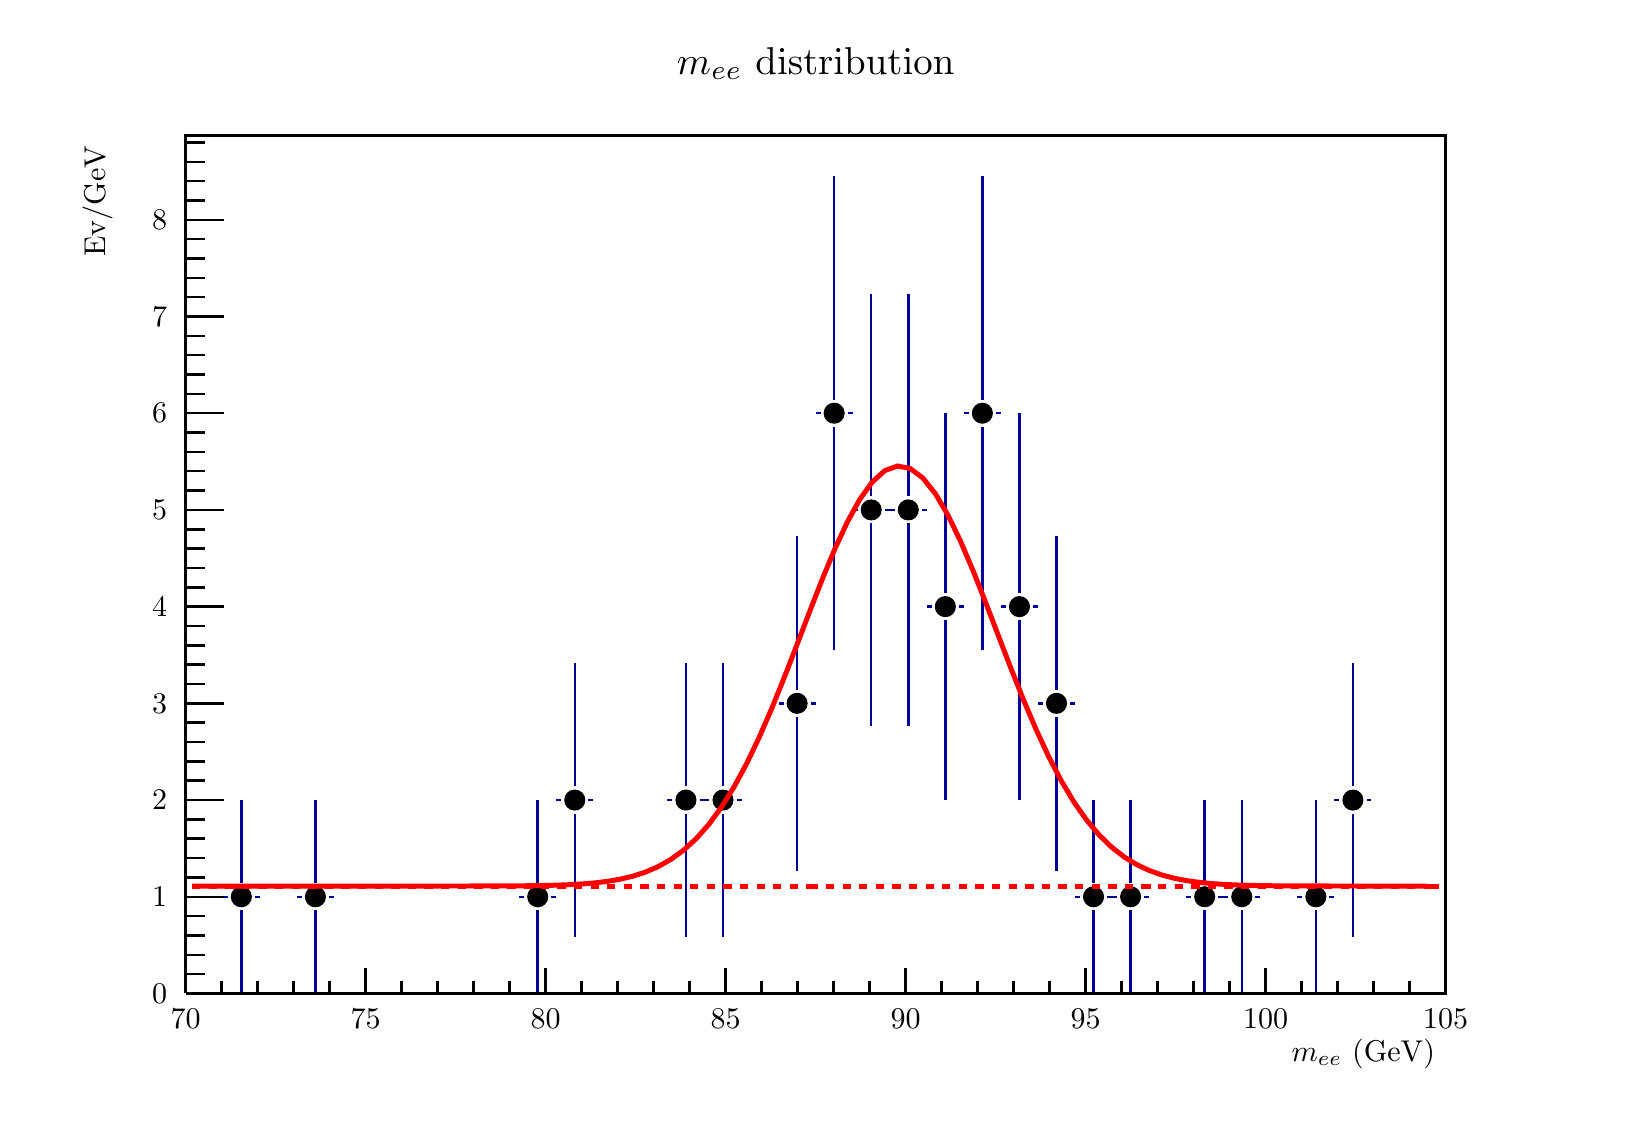
\begin{tikzpicture}
\pgfdeclareplotmark{cross} {
\pgfpathmoveto{\pgfpoint{-0.3\pgfplotmarksize}{\pgfplotmarksize}}
\pgfpathlineto{\pgfpoint{+0.3\pgfplotmarksize}{\pgfplotmarksize}}
\pgfpathlineto{\pgfpoint{+0.3\pgfplotmarksize}{0.3\pgfplotmarksize}}
\pgfpathlineto{\pgfpoint{+1\pgfplotmarksize}{0.3\pgfplotmarksize}}
\pgfpathlineto{\pgfpoint{+1\pgfplotmarksize}{-0.3\pgfplotmarksize}}
\pgfpathlineto{\pgfpoint{+0.3\pgfplotmarksize}{-0.3\pgfplotmarksize}}
\pgfpathlineto{\pgfpoint{+0.3\pgfplotmarksize}{-1.\pgfplotmarksize}}
\pgfpathlineto{\pgfpoint{-0.3\pgfplotmarksize}{-1.\pgfplotmarksize}}
\pgfpathlineto{\pgfpoint{-0.3\pgfplotmarksize}{-0.3\pgfplotmarksize}}
\pgfpathlineto{\pgfpoint{-1.\pgfplotmarksize}{-0.3\pgfplotmarksize}}
\pgfpathlineto{\pgfpoint{-1.\pgfplotmarksize}{0.3\pgfplotmarksize}}
\pgfpathlineto{\pgfpoint{-0.3\pgfplotmarksize}{0.3\pgfplotmarksize}}
\pgfpathclose
\pgfusepathqstroke
}
\pgfdeclareplotmark{cross*} {
\pgfpathmoveto{\pgfpoint{-0.3\pgfplotmarksize}{\pgfplotmarksize}}
\pgfpathlineto{\pgfpoint{+0.3\pgfplotmarksize}{\pgfplotmarksize}}
\pgfpathlineto{\pgfpoint{+0.3\pgfplotmarksize}{0.3\pgfplotmarksize}}
\pgfpathlineto{\pgfpoint{+1\pgfplotmarksize}{0.3\pgfplotmarksize}}
\pgfpathlineto{\pgfpoint{+1\pgfplotmarksize}{-0.3\pgfplotmarksize}}
\pgfpathlineto{\pgfpoint{+0.3\pgfplotmarksize}{-0.3\pgfplotmarksize}}
\pgfpathlineto{\pgfpoint{+0.3\pgfplotmarksize}{-1.\pgfplotmarksize}}
\pgfpathlineto{\pgfpoint{-0.3\pgfplotmarksize}{-1.\pgfplotmarksize}}
\pgfpathlineto{\pgfpoint{-0.3\pgfplotmarksize}{-0.3\pgfplotmarksize}}
\pgfpathlineto{\pgfpoint{-1.\pgfplotmarksize}{-0.3\pgfplotmarksize}}
\pgfpathlineto{\pgfpoint{-1.\pgfplotmarksize}{0.3\pgfplotmarksize}}
\pgfpathlineto{\pgfpoint{-0.3\pgfplotmarksize}{0.3\pgfplotmarksize}}
\pgfpathclose
\pgfusepathqfillstroke
}
\pgfdeclareplotmark{newstar} {
\pgfpathmoveto{\pgfqpoint{0pt}{\pgfplotmarksize}}
\pgfpathlineto{\pgfqpointpolar{44}{0.5\pgfplotmarksize}}
\pgfpathlineto{\pgfqpointpolar{18}{\pgfplotmarksize}}
\pgfpathlineto{\pgfqpointpolar{-20}{0.5\pgfplotmarksize}}
\pgfpathlineto{\pgfqpointpolar{-54}{\pgfplotmarksize}}
\pgfpathlineto{\pgfqpointpolar{-90}{0.5\pgfplotmarksize}}
\pgfpathlineto{\pgfqpointpolar{234}{\pgfplotmarksize}}
\pgfpathlineto{\pgfqpointpolar{198}{0.5\pgfplotmarksize}}
\pgfpathlineto{\pgfqpointpolar{162}{\pgfplotmarksize}}
\pgfpathlineto{\pgfqpointpolar{134}{0.5\pgfplotmarksize}}
\pgfpathclose
\pgfusepathqstroke
}
\pgfdeclareplotmark{newstar*} {
\pgfpathmoveto{\pgfqpoint{0pt}{\pgfplotmarksize}}
\pgfpathlineto{\pgfqpointpolar{44}{0.5\pgfplotmarksize}}
\pgfpathlineto{\pgfqpointpolar{18}{\pgfplotmarksize}}
\pgfpathlineto{\pgfqpointpolar{-20}{0.5\pgfplotmarksize}}
\pgfpathlineto{\pgfqpointpolar{-54}{\pgfplotmarksize}}
\pgfpathlineto{\pgfqpointpolar{-90}{0.5\pgfplotmarksize}}
\pgfpathlineto{\pgfqpointpolar{234}{\pgfplotmarksize}}
\pgfpathlineto{\pgfqpointpolar{198}{0.5\pgfplotmarksize}}
\pgfpathlineto{\pgfqpointpolar{162}{\pgfplotmarksize}}
\pgfpathlineto{\pgfqpointpolar{134}{0.5\pgfplotmarksize}}
\pgfpathclose
\pgfusepathqfillstroke
}
\definecolor{c}{rgb}{1,1,1};
\draw [color=c, fill=c] (0,0) rectangle (20,13.6207);
\draw [color=c, fill=c] (2,1.36207) rectangle (18,12.2586);
\definecolor{c}{rgb}{0,0,0};
\draw [c,line width=0.9] (2,1.36207) -- (2,12.2586) -- (18,12.2586) -- (18,1.36207) -- (2,1.36207);
\definecolor{c}{rgb}{1,1,1};
\draw [color=c, fill=c] (2,1.36207) rectangle (18,12.2586);
\definecolor{c}{rgb}{0,0,0};
\draw [c,line width=0.9] (2,1.36207) -- (2,12.2586) -- (18,12.2586) -- (18,1.36207) -- (2,1.36207);
\definecolor{c}{rgb}{0,0,0.6};
\draw [c,line width=0.9] (2.70588,1.36207) -- (2.70588,2.41786);
\draw [c,line width=0.9] (2.70588,2.76268) -- (2.70588,3.81847);
\draw [c,line width=0.9] (2.47059,2.59027) -- (2.53347,2.59027);
\draw [c,line width=0.9] (2.8783,2.59027) -- (2.94118,2.59027);
\definecolor{c}{rgb}{0,0,0};
\foreach \P in {(2.70588,2.59027)}{\draw[mark options={color=c,fill=c},mark size=3.603604pt,mark=*] plot coordinates {\P};}
\definecolor{c}{rgb}{0,0,0.6};
\draw [c,line width=0.9] (3.64706,1.36207) -- (3.64706,2.41786);
\draw [c,line width=0.9] (3.64706,2.76268) -- (3.64706,3.81847);
\draw [c,line width=0.9] (3.41176,2.59027) -- (3.47465,2.59027);
\draw [c,line width=0.9] (3.81947,2.59027) -- (3.88235,2.59027);
\definecolor{c}{rgb}{0,0,0};
\foreach \P in {(3.64706,2.59027)}{\draw[mark options={color=c,fill=c},mark size=3.603604pt,mark=*] plot coordinates {\P};}
\definecolor{c}{rgb}{0,0,0.6};
\draw [c,line width=0.9] (6.47059,1.36207) -- (6.47059,2.41786);
\draw [c,line width=0.9] (6.47059,2.76268) -- (6.47059,3.81847);
\draw [c,line width=0.9] (6.23529,2.59027) -- (6.29817,2.59027);
\draw [c,line width=0.9] (6.643,2.59027) -- (6.70588,2.59027);
\definecolor{c}{rgb}{0,0,0};
\foreach \P in {(6.47059,2.59027)}{\draw[mark options={color=c,fill=c},mark size=3.603604pt,mark=*] plot coordinates {\P};}
\definecolor{c}{rgb}{0,0,0.6};
\draw [c,line width=0.9] (6.94118,2.08153) -- (6.94118,3.64606);
\draw [c,line width=0.9] (6.94118,3.99088) -- (6.94118,5.55541);
\draw [c,line width=0.9] (6.70588,3.81847) -- (6.76876,3.81847);
\draw [c,line width=0.9] (7.11359,3.81847) -- (7.17647,3.81847);
\definecolor{c}{rgb}{0,0,0};
\foreach \P in {(6.94118,3.81847)}{\draw[mark options={color=c,fill=c},mark size=3.603604pt,mark=*] plot coordinates {\P};}
\definecolor{c}{rgb}{0,0,0.6};
\draw [c,line width=0.9] (8.35294,2.08153) -- (8.35294,3.64606);
\draw [c,line width=0.9] (8.35294,3.99088) -- (8.35294,5.55541);
\draw [c,line width=0.9] (8.11765,3.81847) -- (8.18053,3.81847);
\draw [c,line width=0.9] (8.52536,3.81847) -- (8.58823,3.81847);
\definecolor{c}{rgb}{0,0,0};
\foreach \P in {(8.35294,3.81847)}{\draw[mark options={color=c,fill=c},mark size=3.603604pt,mark=*] plot coordinates {\P};}
\definecolor{c}{rgb}{0,0,0.6};
\draw [c,line width=0.9] (8.82353,2.08153) -- (8.82353,3.64606);
\draw [c,line width=0.9] (8.82353,3.99088) -- (8.82353,5.55541);
\draw [c,line width=0.9] (8.58823,3.81847) -- (8.65112,3.81847);
\draw [c,line width=0.9] (8.99594,3.81847) -- (9.05882,3.81847);
\definecolor{c}{rgb}{0,0,0};
\foreach \P in {(8.82353,3.81847)}{\draw[mark options={color=c,fill=c},mark size=3.603604pt,mark=*] plot coordinates {\P};}
\definecolor{c}{rgb}{0,0,0.6};
\draw [c,line width=0.9] (9.76471,2.91936) -- (9.76471,4.87426);
\draw [c,line width=0.9] (9.76471,5.21908) -- (9.76471,7.17398);
\draw [c,line width=0.9] (9.52941,5.04667) -- (9.59229,5.04667);
\draw [c,line width=0.9] (9.93712,5.04667) -- (10,5.04667);
\definecolor{c}{rgb}{0,0,0};
\foreach \P in {(9.76471,5.04667)}{\draw[mark options={color=c,fill=c},mark size=3.603604pt,mark=*] plot coordinates {\P};}
\definecolor{c}{rgb}{0,0,0.6};
\draw [c,line width=0.9] (10.2353,5.72281) -- (10.2353,8.55886);
\draw [c,line width=0.9] (10.2353,8.90369) -- (10.2353,11.7397);
\draw [c,line width=0.9] (10,8.73127) -- (10.0629,8.73127);
\draw [c,line width=0.9] (10.4077,8.73127) -- (10.4706,8.73127);
\definecolor{c}{rgb}{0,0,0};
\foreach \P in {(10.2353,8.73127)}{\draw[mark options={color=c,fill=c},mark size=3.603604pt,mark=*] plot coordinates {\P};}
\definecolor{c}{rgb}{0,0,0.6};
\draw [c,line width=0.9] (10.7059,4.75673) -- (10.7059,7.33066);
\draw [c,line width=0.9] (10.7059,7.67549) -- (10.7059,10.2494);
\draw [c,line width=0.9] (10.4706,7.50307) -- (10.5335,7.50307);
\draw [c,line width=0.9] (10.8783,7.50307) -- (10.9412,7.50307);
\definecolor{c}{rgb}{0,0,0};
\foreach \P in {(10.7059,7.50307)}{\draw[mark options={color=c,fill=c},mark size=3.603604pt,mark=*] plot coordinates {\P};}
\definecolor{c}{rgb}{0,0,0.6};
\draw [c,line width=0.9] (11.1765,4.75673) -- (11.1765,7.33066);
\draw [c,line width=0.9] (11.1765,7.67549) -- (11.1765,10.2494);
\draw [c,line width=0.9] (10.9412,7.50307) -- (11.0041,7.50307);
\draw [c,line width=0.9] (11.3489,7.50307) -- (11.4118,7.50307);
\definecolor{c}{rgb}{0,0,0};
\foreach \P in {(11.1765,7.50307)}{\draw[mark options={color=c,fill=c},mark size=3.603604pt,mark=*] plot coordinates {\P};}
\definecolor{c}{rgb}{0,0,0.6};
\draw [c,line width=0.9] (11.6471,3.81847) -- (11.6471,6.10246);
\draw [c,line width=0.9] (11.6471,6.44729) -- (11.6471,8.73127);
\draw [c,line width=0.9] (11.4118,6.27487) -- (11.4746,6.27487);
\draw [c,line width=0.9] (11.8195,6.27487) -- (11.8824,6.27487);
\definecolor{c}{rgb}{0,0,0};
\foreach \P in {(11.6471,6.27487)}{\draw[mark options={color=c,fill=c},mark size=3.603604pt,mark=*] plot coordinates {\P};}
\definecolor{c}{rgb}{0,0,0.6};
\draw [c,line width=0.9] (12.1176,5.72281) -- (12.1176,8.55886);
\draw [c,line width=0.9] (12.1176,8.90369) -- (12.1176,11.7397);
\draw [c,line width=0.9] (11.8824,8.73127) -- (11.9452,8.73127);
\draw [c,line width=0.9] (12.2901,8.73127) -- (12.3529,8.73127);
\definecolor{c}{rgb}{0,0,0};
\foreach \P in {(12.1176,8.73127)}{\draw[mark options={color=c,fill=c},mark size=3.603604pt,mark=*] plot coordinates {\P};}
\definecolor{c}{rgb}{0,0,0.6};
\draw [c,line width=0.9] (12.5882,3.81847) -- (12.5882,6.10246);
\draw [c,line width=0.9] (12.5882,6.44729) -- (12.5882,8.73127);
\draw [c,line width=0.9] (12.3529,6.27487) -- (12.4158,6.27487);
\draw [c,line width=0.9] (12.7606,6.27487) -- (12.8235,6.27487);
\definecolor{c}{rgb}{0,0,0};
\foreach \P in {(12.5882,6.27487)}{\draw[mark options={color=c,fill=c},mark size=3.603604pt,mark=*] plot coordinates {\P};}
\definecolor{c}{rgb}{0,0,0.6};
\draw [c,line width=0.9] (13.0588,2.91936) -- (13.0588,4.87426);
\draw [c,line width=0.9] (13.0588,5.21908) -- (13.0588,7.17398);
\draw [c,line width=0.9] (12.8235,5.04667) -- (12.8864,5.04667);
\draw [c,line width=0.9] (13.2312,5.04667) -- (13.2941,5.04667);
\definecolor{c}{rgb}{0,0,0};
\foreach \P in {(13.0588,5.04667)}{\draw[mark options={color=c,fill=c},mark size=3.603604pt,mark=*] plot coordinates {\P};}
\definecolor{c}{rgb}{0,0,0.6};
\draw [c,line width=0.9] (13.5294,1.36207) -- (13.5294,2.41786);
\draw [c,line width=0.9] (13.5294,2.76268) -- (13.5294,3.81847);
\draw [c,line width=0.9] (13.2941,2.59027) -- (13.357,2.59027);
\draw [c,line width=0.9] (13.7018,2.59027) -- (13.7647,2.59027);
\definecolor{c}{rgb}{0,0,0};
\foreach \P in {(13.5294,2.59027)}{\draw[mark options={color=c,fill=c},mark size=3.603604pt,mark=*] plot coordinates {\P};}
\definecolor{c}{rgb}{0,0,0.6};
\draw [c,line width=0.9] (14,1.36207) -- (14,2.41786);
\draw [c,line width=0.9] (14,2.76268) -- (14,3.81847);
\draw [c,line width=0.9] (13.7647,2.59027) -- (13.8276,2.59027);
\draw [c,line width=0.9] (14.1724,2.59027) -- (14.2353,2.59027);
\definecolor{c}{rgb}{0,0,0};
\foreach \P in {(14,2.59027)}{\draw[mark options={color=c,fill=c},mark size=3.603604pt,mark=*] plot coordinates {\P};}
\definecolor{c}{rgb}{0,0,0.6};
\draw [c,line width=0.9] (14.9412,1.36207) -- (14.9412,2.41786);
\draw [c,line width=0.9] (14.9412,2.76268) -- (14.9412,3.81847);
\draw [c,line width=0.9] (14.7059,2.59027) -- (14.7688,2.59027);
\draw [c,line width=0.9] (15.1136,2.59027) -- (15.1765,2.59027);
\definecolor{c}{rgb}{0,0,0};
\foreach \P in {(14.9412,2.59027)}{\draw[mark options={color=c,fill=c},mark size=3.603604pt,mark=*] plot coordinates {\P};}
\definecolor{c}{rgb}{0,0,0.6};
\draw [c,line width=0.9] (15.4118,1.36207) -- (15.4118,2.41786);
\draw [c,line width=0.9] (15.4118,2.76268) -- (15.4118,3.81847);
\draw [c,line width=0.9] (15.1765,2.59027) -- (15.2394,2.59027);
\draw [c,line width=0.9] (15.5842,2.59027) -- (15.6471,2.59027);
\definecolor{c}{rgb}{0,0,0};
\foreach \P in {(15.4118,2.59027)}{\draw[mark options={color=c,fill=c},mark size=3.603604pt,mark=*] plot coordinates {\P};}
\definecolor{c}{rgb}{0,0,0.6};
\draw [c,line width=0.9] (16.3529,1.36207) -- (16.3529,2.41786);
\draw [c,line width=0.9] (16.3529,2.76268) -- (16.3529,3.81847);
\draw [c,line width=0.9] (16.1176,2.59027) -- (16.1805,2.59027);
\draw [c,line width=0.9] (16.5254,2.59027) -- (16.5882,2.59027);
\definecolor{c}{rgb}{0,0,0};
\foreach \P in {(16.3529,2.59027)}{\draw[mark options={color=c,fill=c},mark size=3.603604pt,mark=*] plot coordinates {\P};}
\definecolor{c}{rgb}{0,0,0.6};
\draw [c,line width=0.9] (16.8235,2.08153) -- (16.8235,3.64606);
\draw [c,line width=0.9] (16.8235,3.99088) -- (16.8235,5.55541);
\draw [c,line width=0.9] (16.5882,3.81847) -- (16.6511,3.81847);
\draw [c,line width=0.9] (16.9959,3.81847) -- (17.0588,3.81847);
\definecolor{c}{rgb}{0,0,0};
\foreach \P in {(16.8235,3.81847)}{\draw[mark options={color=c,fill=c},mark size=3.603604pt,mark=*] plot coordinates {\P};}
\definecolor{c}{rgb}{1,0,0};
\draw [c,line width=1.8] (2.08,2.72674) -- (2.24,2.72674) -- (2.4,2.72674) -- (2.56,2.72674) -- (2.72,2.72674) -- (2.88,2.72674) -- (3.04,2.72674) -- (3.2,2.72674) -- (3.36,2.72674) -- (3.52,2.72674) -- (3.68,2.72674) -- (3.84,2.72674) -- (4,2.72674)
 -- (4.16,2.72674) -- (4.32,2.72674) -- (4.48,2.72674) -- (4.64,2.72674) -- (4.8,2.72675) -- (4.96,2.72676) -- (5.12,2.72679) -- (5.28,2.72683) -- (5.44,2.72691) -- (5.6,2.72704) -- (5.76,2.72727) -- (5.92,2.72765) -- (6.08,2.7283) -- (6.24,2.72935)
 -- (6.4,2.73103) -- (6.56,2.73367) -- (6.72,2.73777) -- (6.88,2.74398) -- (7.04,2.75325) -- (7.2,2.76683) -- (7.36,2.78635) -- (7.52,2.8139) -- (7.68,2.85206) -- (7.84,2.90394) -- (8,2.97311) -- (8.16,3.06359) -- (8.32,3.17964) -- (8.48,3.32554) --
 (8.64,3.50528) -- (8.8,3.72212) -- (8.96,3.97819) -- (9.12,4.27397) -- (9.28,4.60784) -- (9.44,4.97571) -- (9.6,5.37079) -- (9.76,5.78358) -- (9.92,6.20202);
\draw [c,line width=1.8] (9.92,6.20202) -- (10.08,6.61202) -- (10.24,6.99814) -- (10.4,7.34452) -- (10.56,7.63595) -- (10.72,7.85897) -- (10.88,8.00287) -- (11.04,8.06058) -- (11.2,8.02923) -- (11.36,7.91038) -- (11.52,7.70991) -- (11.68,7.43751) --
 (11.84,7.10592) -- (12,6.72996) -- (12.16,6.32541) -- (12.32,5.90792) -- (12.48,5.4921) -- (12.64,5.09064) -- (12.8,4.71385) -- (12.96,4.36934) -- (13.12,4.06196) -- (13.28,3.79406) -- (13.44,3.56571) -- (13.6,3.37525) -- (13.76,3.21969) --
 (13.92,3.09521) -- (14.08,2.99758) -- (14.24,2.92251) -- (14.4,2.86589) -- (14.56,2.824) -- (14.72,2.79359) -- (14.88,2.77193) -- (15.04,2.75677) -- (15.2,2.74637) -- (15.36,2.73935) -- (15.52,2.73471) -- (15.68,2.73169) -- (15.84,2.72977) --
 (16,2.72856) -- (16.16,2.72781) -- (16.32,2.72736) -- (16.48,2.72709) -- (16.64,2.72694) -- (16.8,2.72685) -- (16.96,2.7268) -- (17.12,2.72677) -- (17.28,2.72675) -- (17.44,2.72675) -- (17.6,2.72674) -- (17.76,2.72674);
\draw [c,line width=1.8] (17.76,2.72674) -- (17.92,2.72674);
\definecolor{c}{rgb}{0,0,0};
\draw [c,line width=0.9] (2,1.36207) -- (18,1.36207);
\draw [anchor= east] (18,0.59931) node[scale=1.08496, color=c, rotate=0]{$m_{ee} \mbox{ (GeV)}$};
\draw [c,line width=0.9] (2,1.68897) -- (2,1.36207);
\draw [c,line width=0.9] (2.45714,1.52552) -- (2.45714,1.36207);
\draw [c,line width=0.9] (2.91429,1.52552) -- (2.91429,1.36207);
\draw [c,line width=0.9] (3.37143,1.52552) -- (3.37143,1.36207);
\draw [c,line width=0.9] (3.82857,1.52552) -- (3.82857,1.36207);
\draw [c,line width=0.9] (4.28571,1.68897) -- (4.28571,1.36207);
\draw [c,line width=0.9] (4.74286,1.52552) -- (4.74286,1.36207);
\draw [c,line width=0.9] (5.2,1.52552) -- (5.2,1.36207);
\draw [c,line width=0.9] (5.65714,1.52552) -- (5.65714,1.36207);
\draw [c,line width=0.9] (6.11429,1.52552) -- (6.11429,1.36207);
\draw [c,line width=0.9] (6.57143,1.68897) -- (6.57143,1.36207);
\draw [c,line width=0.9] (7.02857,1.52552) -- (7.02857,1.36207);
\draw [c,line width=0.9] (7.48571,1.52552) -- (7.48571,1.36207);
\draw [c,line width=0.9] (7.94286,1.52552) -- (7.94286,1.36207);
\draw [c,line width=0.9] (8.4,1.52552) -- (8.4,1.36207);
\draw [c,line width=0.9] (8.85714,1.68897) -- (8.85714,1.36207);
\draw [c,line width=0.9] (9.31429,1.52552) -- (9.31429,1.36207);
\draw [c,line width=0.9] (9.77143,1.52552) -- (9.77143,1.36207);
\draw [c,line width=0.9] (10.2286,1.52552) -- (10.2286,1.36207);
\draw [c,line width=0.9] (10.6857,1.52552) -- (10.6857,1.36207);
\draw [c,line width=0.9] (11.1429,1.68897) -- (11.1429,1.36207);
\draw [c,line width=0.9] (11.6,1.52552) -- (11.6,1.36207);
\draw [c,line width=0.9] (12.0571,1.52552) -- (12.0571,1.36207);
\draw [c,line width=0.9] (12.5143,1.52552) -- (12.5143,1.36207);
\draw [c,line width=0.9] (12.9714,1.52552) -- (12.9714,1.36207);
\draw [c,line width=0.9] (13.4286,1.68897) -- (13.4286,1.36207);
\draw [c,line width=0.9] (13.8857,1.52552) -- (13.8857,1.36207);
\draw [c,line width=0.9] (14.3429,1.52552) -- (14.3429,1.36207);
\draw [c,line width=0.9] (14.8,1.52552) -- (14.8,1.36207);
\draw [c,line width=0.9] (15.2571,1.52552) -- (15.2571,1.36207);
\draw [c,line width=0.9] (15.7143,1.68897) -- (15.7143,1.36207);
\draw [c,line width=0.9] (16.1714,1.52552) -- (16.1714,1.36207);
\draw [c,line width=0.9] (16.6286,1.52552) -- (16.6286,1.36207);
\draw [c,line width=0.9] (17.0857,1.52552) -- (17.0857,1.36207);
\draw [c,line width=0.9] (17.5429,1.52552) -- (17.5429,1.36207);
\draw [c,line width=0.9] (18,1.68897) -- (18,1.36207);
\draw [anchor=base] (2,0.912586) node[scale=1.08496, color=c, rotate=0]{70};
\draw [anchor=base] (4.28571,0.912586) node[scale=1.08496, color=c, rotate=0]{75};
\draw [anchor=base] (6.57143,0.912586) node[scale=1.08496, color=c, rotate=0]{80};
\draw [anchor=base] (8.85714,0.912586) node[scale=1.08496, color=c, rotate=0]{85};
\draw [anchor=base] (11.1429,0.912586) node[scale=1.08496, color=c, rotate=0]{90};
\draw [anchor=base] (13.4286,0.912586) node[scale=1.08496, color=c, rotate=0]{95};
\draw [anchor=base] (15.7143,0.912586) node[scale=1.08496, color=c, rotate=0]{100};
\draw [anchor=base] (18,0.912586) node[scale=1.08496, color=c, rotate=0]{105};
\draw [c,line width=0.9] (2,1.36207) -- (2,12.2586);
\draw [anchor= east] (0.88,12.2586) node[scale=1.08496, color=c, rotate=90]{$\mbox{Ev/GeV}$};
\draw [c,line width=0.9] (2.48,1.36207) -- (2,1.36207);
\draw [c,line width=0.9] (2.24,1.60771) -- (2,1.60771);
\draw [c,line width=0.9] (2.24,1.85335) -- (2,1.85335);
\draw [c,line width=0.9] (2.24,2.09899) -- (2,2.09899);
\draw [c,line width=0.9] (2.24,2.34463) -- (2,2.34463);
\draw [c,line width=0.9] (2.48,2.59027) -- (2,2.59027);
\draw [c,line width=0.9] (2.24,2.83591) -- (2,2.83591);
\draw [c,line width=0.9] (2.24,3.08155) -- (2,3.08155);
\draw [c,line width=0.9] (2.24,3.32719) -- (2,3.32719);
\draw [c,line width=0.9] (2.24,3.57283) -- (2,3.57283);
\draw [c,line width=0.9] (2.48,3.81847) -- (2,3.81847);
\draw [c,line width=0.9] (2.24,4.06411) -- (2,4.06411);
\draw [c,line width=0.9] (2.24,4.30975) -- (2,4.30975);
\draw [c,line width=0.9] (2.24,4.55539) -- (2,4.55539);
\draw [c,line width=0.9] (2.24,4.80103) -- (2,4.80103);
\draw [c,line width=0.9] (2.48,5.04667) -- (2,5.04667);
\draw [c,line width=0.9] (2.24,5.29231) -- (2,5.29231);
\draw [c,line width=0.9] (2.24,5.53795) -- (2,5.53795);
\draw [c,line width=0.9] (2.24,5.78359) -- (2,5.78359);
\draw [c,line width=0.9] (2.24,6.02923) -- (2,6.02923);
\draw [c,line width=0.9] (2.48,6.27487) -- (2,6.27487);
\draw [c,line width=0.9] (2.24,6.52051) -- (2,6.52051);
\draw [c,line width=0.9] (2.24,6.76615) -- (2,6.76615);
\draw [c,line width=0.9] (2.24,7.01179) -- (2,7.01179);
\draw [c,line width=0.9] (2.24,7.25743) -- (2,7.25743);
\draw [c,line width=0.9] (2.48,7.50307) -- (2,7.50307);
\draw [c,line width=0.9] (2.24,7.74871) -- (2,7.74871);
\draw [c,line width=0.9] (2.24,7.99435) -- (2,7.99435);
\draw [c,line width=0.9] (2.24,8.23999) -- (2,8.23999);
\draw [c,line width=0.9] (2.24,8.48563) -- (2,8.48563);
\draw [c,line width=0.9] (2.48,8.73127) -- (2,8.73127);
\draw [c,line width=0.9] (2.24,8.97691) -- (2,8.97691);
\draw [c,line width=0.9] (2.24,9.22255) -- (2,9.22255);
\draw [c,line width=0.9] (2.24,9.46819) -- (2,9.46819);
\draw [c,line width=0.9] (2.24,9.71383) -- (2,9.71383);
\draw [c,line width=0.9] (2.48,9.95947) -- (2,9.95947);
\draw [c,line width=0.9] (2.24,10.2051) -- (2,10.2051);
\draw [c,line width=0.9] (2.24,10.4508) -- (2,10.4508);
\draw [c,line width=0.9] (2.24,10.6964) -- (2,10.6964);
\draw [c,line width=0.9] (2.24,10.942) -- (2,10.942);
\draw [c,line width=0.9] (2.48,11.1877) -- (2,11.1877);
\draw [c,line width=0.9] (2.48,11.1877) -- (2,11.1877);
\draw [c,line width=0.9] (2.24,11.4333) -- (2,11.4333);
\draw [c,line width=0.9] (2.24,11.679) -- (2,11.679);
\draw [c,line width=0.9] (2.24,11.9246) -- (2,11.9246);
\draw [c,line width=0.9] (2.24,12.1702) -- (2,12.1702);
\draw [anchor= east] (1.9,1.36207) node[scale=1.08496, color=c, rotate=0]{0};
\draw [anchor= east] (1.9,2.59027) node[scale=1.08496, color=c, rotate=0]{1};
\draw [anchor= east] (1.9,3.81847) node[scale=1.08496, color=c, rotate=0]{2};
\draw [anchor= east] (1.9,5.04667) node[scale=1.08496, color=c, rotate=0]{3};
\draw [anchor= east] (1.9,6.27487) node[scale=1.08496, color=c, rotate=0]{4};
\draw [anchor= east] (1.9,7.50307) node[scale=1.08496, color=c, rotate=0]{5};
\draw [anchor= east] (1.9,8.73127) node[scale=1.08496, color=c, rotate=0]{6};
\draw [anchor= east] (1.9,9.95947) node[scale=1.08496, color=c, rotate=0]{7};
\draw [anchor= east] (1.9,11.1877) node[scale=1.08496, color=c, rotate=0]{8};
\definecolor{c}{rgb}{1,0,0};
\draw [c,dashed,line width=1.8] (2.08,2.72674) -- (2.24,2.72674) -- (2.4,2.72674) -- (2.56,2.72674) -- (2.72,2.72674) -- (2.88,2.72674) -- (3.04,2.72674) -- (3.2,2.72674) -- (3.36,2.72674) -- (3.52,2.72674) -- (3.68,2.72674) -- (3.84,2.72674) --
 (4,2.72674) -- (4.16,2.72674) -- (4.32,2.72674) -- (4.48,2.72674) -- (4.64,2.72674) -- (4.8,2.72674) -- (4.96,2.72674) -- (5.12,2.72674) -- (5.28,2.72674) -- (5.44,2.72674) -- (5.6,2.72674) -- (5.76,2.72674) -- (5.92,2.72674) -- (6.08,2.72674) --
 (6.24,2.72674) -- (6.4,2.72674) -- (6.56,2.72674) -- (6.72,2.72674) -- (6.88,2.72674) -- (7.04,2.72674) -- (7.2,2.72674) -- (7.36,2.72674) -- (7.52,2.72674) -- (7.68,2.72674) -- (7.84,2.72674) -- (8,2.72674) -- (8.16,2.72674) -- (8.32,2.72674) --
 (8.48,2.72674) -- (8.64,2.72674) -- (8.8,2.72674) -- (8.96,2.72674) -- (9.12,2.72674) -- (9.28,2.72674) -- (9.44,2.72674) -- (9.6,2.72674) -- (9.76,2.72674) -- (9.92,2.72674);
\draw [c,dashed,line width=1.8] (9.92,2.72674) -- (10.08,2.72674) -- (10.24,2.72674) -- (10.4,2.72674) -- (10.56,2.72674) -- (10.72,2.72674) -- (10.88,2.72674) -- (11.04,2.72674) -- (11.2,2.72674) -- (11.36,2.72674) -- (11.52,2.72674) --
 (11.68,2.72674) -- (11.84,2.72674) -- (12,2.72674) -- (12.16,2.72674) -- (12.32,2.72674) -- (12.48,2.72674) -- (12.64,2.72674) -- (12.8,2.72674) -- (12.96,2.72674) -- (13.12,2.72674) -- (13.28,2.72674) -- (13.44,2.72674) -- (13.6,2.72674) --
 (13.76,2.72674) -- (13.92,2.72674) -- (14.08,2.72674) -- (14.24,2.72674) -- (14.4,2.72674) -- (14.56,2.72674) -- (14.72,2.72674) -- (14.88,2.72674) -- (15.04,2.72674) -- (15.2,2.72674) -- (15.36,2.72674) -- (15.52,2.72674) -- (15.68,2.72674) --
 (15.84,2.72674) -- (16,2.72674) -- (16.16,2.72674) -- (16.32,2.72674) -- (16.48,2.72674) -- (16.64,2.72674) -- (16.8,2.72674) -- (16.96,2.72674) -- (17.12,2.72674) -- (17.28,2.72674) -- (17.44,2.72674) -- (17.6,2.72674) -- (17.76,2.72674);
\draw [c,dashed,line width=1.8] (17.76,2.72674) -- (17.92,2.72674);
\definecolor{c}{rgb}{0,0,0};
\draw (10,13.1733) node[scale=1.40406, color=c, rotate=0]{$m_{ee} \mbox{ distribution}$};
\end{tikzpicture}
